\begin{tcolorbox}
Die Produktfunktionen beschreiben jede einzelne Funktion des Produkts mittels Anwendungsfalldiagrammen und Anwendungsfalltabellen.
Diese sollen möglichst ausschlaggebend für das zu entwickelnde System sein und nicht simple Produktfunktionen wie z.B. Login, Account erstellen, Gruppe beitreten, Passwort ändern oder ähnliches zeigen.
\autoref{fig:anwendungsfall-app-tabelle-xx-1} stellt eine exemplarische Tabelle für die Beschreibung eines Anwendungsfalls dar. Stil und Formatierung sind variabel. Nicht jede Zelle muss immer gefüllt sein.
\\\\
In  Tabelle~\autoref{fig:akteur-tabelle} werden alle auftretenden Akteure beschrieben.


\end{tcolorbox}

\begin{figure}[h]
	\centering

	\begin{tabularx}{\textwidth}{ p{.2\textwidth} | p{.2\textwidth} | X }
		\textbf{Akteur} & \textbf{Beschreibung} & \textbf{Verwendet in Anwendungsszenario} \\ \hline
		Informatiker & Programmiert tolle Sachen & Programmieren, Kaffee trinken, Schlafen \\ \hline
		AdministratorIn & Anwender der web Applikation & Komposition-\{bearbeiten, erstellen, darstellen \}, Dienst einfügen
	\end{tabularx}

	\caption{Beschreibung der Akteure}
	\label{fig:akteur-tabelle}
\end{figure}


%%%%%%%%%%%%%%%
%% Anwendungsfall 1 %%
%%%%%%%%%%%%%%%

\section{Anwendungsfalldiagramm - App}

\begin{figure}[h]
	\centering
	\missingfigure{Anwendungsfalldiagramm - App}
	\caption{Anwendungsfalldiagramm - App}
	\label{fig:anwendungsfalldiagramm-app}
\end{figure}

\newpage

\begin{figure}[h]
	\centering
	\begin{tabularx}{\textwidth}{ X | X }
		\textbf{Anwendungsfall ID} & XX-1 \\ \hline
		\textbf{Anwendungsfallname} & Hier steht ein Name. \\ \hline
		\textbf{Initiierender Akteur} & Informatiker \\ \hline
		\textbf{Weitere Akteure} & Designer, Techniker  \\ \hline
		\textbf{Kurzbeschreibung} & Hier steht eine Kurzbeschreibung.  \\ \hline
		\textbf{Vorbedingungen} & -  \\ \hline
		\textbf{Nachbedingungen} & Y trifft zu.  \\ \hline
		\textbf{Ablauf} &
			\begin{enumerate}
				\item Erster ganzer Satz.
				\item Zweiter ganzer Satz.
			\end{enumerate} \\ \hline
		\textbf{Alternative} &
				\begin{enumerate}
					\item Erster ganzer Satz.
					\item Zweiter ganzer Satz.
				\end{enumerate}  \\ \hline
		\textbf{Ausnahme} &
				\begin{enumerate}
					\item Erster ganzer Satz.
					\item Zweiter ganzer Satz.
				\end{enumerate}  \\ \hline
		\textbf{Benutzte Anwendungsfälle} & YY-1 (oder Name) \\ \hline
		\textbf{Spezielle Anforderungen} & - \\ \hline
		\textbf{Annahmen} & -
	\end{tabularx}
	\caption{Anwendungsfall XX-1}
	\label{fig:anwendungsfall-app-tabelle-xx-1}
\end{figure}

\newpage


%%%%%%%%%%%%%%%
%% Anwendungsfall 2 %%
%%%%%%%%%%%%%%%

\section{Anwendungsfalldiagramm - Server}

\begin{figure}[h]
	\centering
	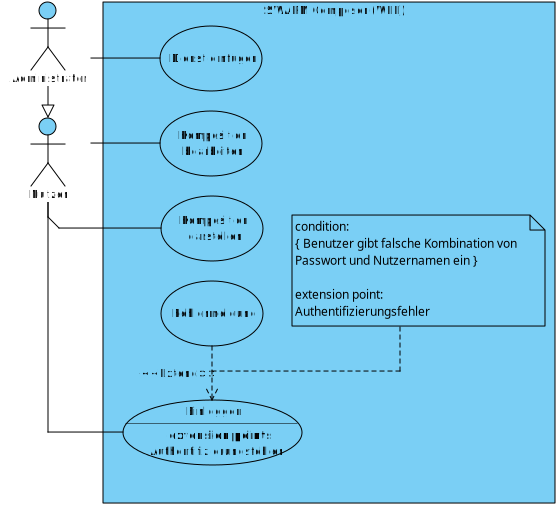
\includegraphics[width=\textwidth]{img/Produktfunktionen_web}
	\caption{Anwendungsfalldiagramm - Server}
	\label{fig:anwendungsfalldiagramm-server}
\end{figure}

\newpage

\begin{figure}[h]
	\centering
	\begin{tabularx}{\textwidth}{ X | X }
		\textbf{Anwendungsfall ID} & WEB-1 \\ \hline
		\textbf{Anwendungsfallname} & Dienst manuell einfügen \\ \hline
		\textbf{Initiierender Akteur} & AdministratorIn \\ \hline
		\textbf{Weitere Akteure} & - \\ \hline
		\textbf{Kurzbeschreibung} & Ein neuer Dienst wird in die Datenbank eingefügt \\ \hline
		\textbf{Vorbedingungen} & AdministratorIn ist eingeloggt und befindet sich auf Administrationsseite \\ \hline
		\textbf{Nachbedingungen} & Neuer Dienst wurde in Datenbank gespeichert \\ \hline
		\textbf{Ablauf} &
		\begin{enumerate}
			\item [1.] [Use-Case: Authentifizieren]
			\item [2.] AdministratorIn wählt Dienst eingeben aus.
			\item [3.] AdministratorIn gibt Dienstdetails in Eingabemaske ein.
			\item [4.] AdministratorIn bestätigt seine Eingabe.
			\item [5.] System akzeptiert Eingabe und speichert in Datenbank.
			\item [6.] Zurück zur Administrationsseite.
		\end{enumerate} \\ \hline
		\textbf{Alternative} & - \\ \hline
		\textbf{Ausnahme} &
		\begin{enumerate}
			\item [1.] [Use-Case: Authentifizieren]
			\item [2.] AdministratorIn wählt Dienst eingeben aus.
			\item [3.] AdministratorIn gibt Dienstdetails in Eingabemaske ein.
			\item [4.] AdministratorIn bestätigt seine Eingabe.
			\item [5.] System akzeptiert Eingabe nicht, da invalide Eingabe.
			\item [6.] System zeigt Fehler und markiert invalide Felder.
			\item [7.] bleibe in der Eingabemaske.
		\end{enumerate} \\ \hline
		\textbf{Benutzte Anwendungsfälle} & - \\ \hline
		\textbf{Spezielle Anforderungen} & - \\ \hline
		\textbf{Annahmen} & -
	\end{tabularx}
	\caption{Anwendungsfall WEB-1}
	\label{fig:anwendungsfall-server-tabelle-web-1}
\end{figure}

\begin{figure}[h]
	\centering
	\begin{tabularx}{\textwidth}{ X | X }
		\textbf{Anwendungsfall ID} & WEB-2 \\ \hline
		\textbf{Anwendungsfallname} & Dienste einlesen. \\ \hline
		\textbf{Initiierender Akteur} & AdministratorIn \\ \hline
		\textbf{Weitere Akteure} & - \\ \hline
		\textbf{Kurzbeschreibung} & Ein oder mehrere Dienste werden über eine Nutzerrechner lokal befindliche JSON Datei eingelesen \\ \hline
		\textbf{Vorbedingungen} & AdministratorIn ist eingeloggt und befindet sich auf Administrationsseite \\ \hline
		\textbf{Nachbedingungen} & Neue Dienst(e) wurden der Datenbank hinzugefügt \\ \hline
		\textbf{Ablauf} &
		\begin{enumerate}
			\item [1.] [Use-Case: Authentifizieren]
			\item [2.] AdministratorIn wählt "Dienste einlesen"-Button aus.
			\item [3.] AdministratorIn wählt hochzuladene JSON Datei aus sich öffnenden Dateibrowser von seinem Rechner aus.
			\item [4.] Eingelesende Daten werden vom System akzeptiert und aufgelistet.
			\item [5.] AdministratorIn drückt Speichern
			\item [6.] Dienste werden in Datenbank gespeichert
			\item [7.] Zurück zur Administrationsseite.
		\end{enumerate} \\ \hline
		\textbf{Alternative} & - \\ \hline
		\textbf{Ausnahme} &
		\begin{enumerate}
			\item [1.]  [Use-Case: Authentifizieren]
			\item [2.]  AdministratorIn wählt "Dienste einlesen"-Button aus.
			\item [3.]  AdministratorIn wählt hochzuladene JSON Datei aus sich öffnenden Dateibrowser von seinem Rechner aus.
			\item [4.]  System erkennt Fehler in der JSON Datei und gibt einen Fehler aus.
			\item [5.]  Administrator bleibt auf der Administrationseite
		\end{enumerate}  \\ \hline
		\textbf{Benutzte Anwendungsfälle} & - \\ \hline
		\textbf{Spezielle Anforderungen} & - \\ \hline
		\textbf{Annahmen} & -
	\end{tabularx}
	\caption{Anwendungsfall WEB-2}
	\label{fig:anwendungsfall-server-tabelle-web-2}
\end{figure}

\begin{figure}[h]
	\centering
	\begin{tabularx}{\textwidth}{ X | X }
		\textbf{Anwendungsfall ID} & WEB-3 \\ \hline
		\textbf{Anwendungsfallname} & Dienst bearbeiten. \\ \hline
		\textbf{Initiierender Akteur} & AdministratorIn \\ \hline
		\textbf{Weitere Akteure} & - \\ \hline
		\textbf{Kurzbeschreibung} & Felder eines existierenden Dienstes werden bearbeitet \\ \hline
		\textbf{Vorbedingungen} & AdministratorIn ist eingeloggt und befindet sich auf Administrationsseite \\ \hline
		\textbf{Nachbedingungen} & Vorgenommende Änderungen am Dienst wurden in Datenbank übernommen \\ \hline
		\textbf{Ablauf} &
		\begin{enumerate}
			\item [1.] [Use-Case: Authentifizieren]
			\item [2.] AdministratorIn wählt Dienst aus Liste von vorhandenen Diensten aus.
			\item [3.] AdministratorIn drückt auf bearbeiten.
			\item [4.] AdministratorIn führt Änderungen in Eingabemaske durch.
			\item [5.] AdministratorIn bestätigt seine Eingabe.
			\item [6.] System akzeptiert änderung und speichert diese in der Datenbank.
		\end{enumerate} \\ \hline
		\textbf{Alternative} & - \\ \hline
		\textbf{Ausnahme} &
		\begin{enumerate}
			\item [1.] [Use-Case: Authentifizieren]
			\item [2.] AdministratorIn wählt Dienst aus Liste von vorhandenen Diensten aus.
			\item [3.] AdministratorIn drückt auf bearbeiten.
			\item [4.] AdministratorIn tätigt eine invalide Eingabe.
			\item [5.] AdministratorIn bestätigt seine Eingabe.
			\item [6.] System erkennt Fehler und zeigt einen Fehler an
			\item [6.] AdministratorIn bleibt auf der Administrationsseite
		\end{enumerate}  \\ \hline
		\textbf{Benutzte Anwendungsfälle} & - \\ \hline
		\textbf{Spezielle Anforderungen} & - \\ \hline
		\textbf{Annahmen} & -
	\end{tabularx}
	\caption{Anwendungsfall WEB-3}
	\label{fig:anwendungsfall-server-tabelle-web-3}
\end{figure}

\begin{figure}[h]
	\centering
	\begin{tabularx}{\textwidth}{ X | X }
		\textbf{Anwendungsfall ID} & WEB-4 \\ \hline
		\textbf{Anwendungsfallname} & Komposition erstellen \\ \hline
		\textbf{Initiierender Akteur} & NutzerIn \\ \hline
		\textbf{Weitere Akteure} & - \\ \hline
		\textbf{Kurzbeschreibung} & Eine neue Komposition wird zum System hinzugefügt. \\ \hline
		\textbf{Vorbedingungen} & NutzerIn befindet sich auf der Übersichtsseite und ist eingeloggt.  \\ \hline
		\textbf{Nachbedingungen} & Komposition ist erstellt und NutzerIn befindet sich im Bearbeitungsmodus. \\ \hline
		\textbf{Ablauf} &
		\begin{enumerate}
			\item[1.]  [Use-Case: Authentifizieren]
			\item[2.]  NutzerIn wählt ``Komposition erstellen'' Option.
			\item[3.]  NutzerIn gibt einen Namen für die Komposition an.
			\item[4.]  NutzerIn wird weitergeleitet zum Bearbeitungsmodus.
		\end{enumerate} \\ \hline
		\textbf{Alternative} & - \\ \hline
		\textbf{Ausnahme} & - \\ \hline
		\textbf{Benutzte Anwendungsfälle} & WEB-5 \\ \hline
		\textbf{Spezielle Anforderungen} & - \\ \hline
		\textbf{Annahmen} & -
	\end{tabularx}
	\caption{Anwendungsfall WEB-5}
	\label{fig:anwendungsfall-server-tabelle-web-4}
\end{figure}

\begin{figure}[h]
	\centering
	\begin{tabularx}{\textwidth}{ X | X }
		\textbf{Anwendungsfall ID} & WEB-5 \\ \hline
		\textbf{Anwendungsfallname} & Komposition bearbeiten \\ \hline
		\textbf{Initiierender Akteur} & NutzerIn \\ \hline
		\textbf{Weitere Akteure} & - \\ \hline
		\textbf{Kurzbeschreibung} & NutzerIn bearbeitet Komposition \\ \hline
		\textbf{Vorbedingungen} & NutzerIn besitzt benötigte Rechte zur Bearbeitung der Komposition und befindet sich auf der Übersichtsseite. \\ \hline
		\textbf{Nachbedingungen} & NutzerIn befindet sich im Bearbeitungsmodus. \\ \hline
		\textbf{Ablauf} &
		\begin{enumerate}
			\item[1.] [Use-Case: Authentifizieren]
			\item[2.] NutzerIn drückt Bearbeitungsbutton bei der Komposition.
			\item[3.] NutzerIn wird in den Bearbeitungsmodus versetzt.
		\end{enumerate} \\ \hline
		\textbf{Alternative} & - \\ \hline
		\textbf{Ausnahme} & - \\ \hline
		\textbf{Benutzte Anwendungsfälle} & - \\ \hline
		\textbf{Spezielle Anforderungen} & - \\ \hline
		\textbf{Annahmen} & Es werden nur Komposition gezeigt für die der NutzerIn die benötigten Rechte besitzt.
                  Der Bearbeitungsbutton ist ausgegraut falls die Bearbeitungsrechte nicht vorhanden sind.
	\end{tabularx}
	\caption{Anwendungsfall WEB-5}
	\label{fig:anwendungsfall-server-tabelle-web-5}
\end{figure}

\begin{figure}[h]
	\centering
	\begin{tabularx}{\textwidth}{ X | X }
		\textbf{Anwendungsfall ID} & WEB-6 \\ \hline
		\textbf{Anwendungsfallname} & Einsehbare Komposition anzeigen \\ \hline
		\textbf{Initiierender Akteur} & unregistrierteR NutzerIn oder NutzerIn \\ \hline
		\textbf{Weitere Akteure} & - \\ \hline
		\textbf{Kurzbeschreibung} & unregistrierteR NutzerIn oder NutzerIn lässt sich eine Komposition anzeigen. \\ \hline
		\textbf{Vorbedingungen} & unregistrierteR NutzerIn oder NutzerIn befindet sich auf der Übersichtsseite. \\ \hline
		\textbf{Nachbedingungen} & unregistrierteR NutzerIn oder NutzerIn wird Komposition angezeigt. \\ \hline
		\textbf{Ablauf} &
		\begin{enumerate}
			\item[1.] [Use-Case: Authentifizieren]
			\item[2.] unregistrierteR NutzerIn oder NutzerIn drückt auf die anzuzeigende Komposition.
			\item[3.] unregistrierteR NutzerIn oder NutzerIn wird die Komposition angezeigt.
		\end{enumerate} \\ \hline
		\textbf{Alternative} & - \\ \hline
		\textbf{Ausnahme} & - \\ \hline
		\textbf{Benutzte Anwendungsfälle} & - \\ \hline
		\textbf{Spezielle Anforderungen} & - \\ \hline
		\textbf{Annahmen} & Es werden nur Kompositionen gezeigt für die der unregistrierteR NutzerIn oder NutzerIn die benötigten Rechte besitzt.
	\end{tabularx}
	\caption{Anwendungsfall WEB-6}
	\label{fig:anwendungsfall-server-tabelle-web-6}
\end{figure}